
\chapter{}

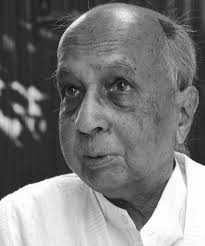
\includegraphics[scale=2]{images/chimu.jpeg}

\noindent
\textbf{ನಾಡೋಜ}\\\textbf{ಡಾ. ಎಂ. ಚಿದಾನಂದ ಮೂರ್ತಿ, ಎಂ.ಎ., ಪಿಎಚ್.ಡಿ. (ಮೈ), ಡಿ.ಲಿಟ್ (ಬೆಂ)}\\\textbf{ವಿಶ್ರಾಂತ ಕನ್ನಡ ಪ್ರಾಧ್ಯಾಪಕರು (ಬೆಂಗಳೂರು ವಿಶ್ವವಿದ್ಯಾಲಯ)}\\\textbf{ಕೇಂದ್ರ ಸಾಹಿತ್ಯ ಅಕಾಡೆಮಿ ಮತ್ತು ಪಂಪ ಪ್ರಶಸ್ತಿ ವಿಜೇತರು}

\vskip.5cm

\noindent
`ಮಿಂಚು' \\ ನಂ.1013/ಬಿ, \\ 4ನೇ ಅಡ್ಡ ರಸ್ತೆ, 11ನೇ ಮುಖ್ಯ ರಸ್ತೆ,\\ ಹಂಪಿ ನಗರ, ಬೆಂಗಳೂರು 560 104,\\ ದೂರವಾಣಿ: 080 - 23300687

\vskip.2cm

ಡಾ. ಎಸ್​. ನಂಜುಂಡಸ್ವಾಮಿಯವರು, ಪಿಎಚ್​.ಡಿ. ಪದವಿಗಾಗಿ, ಡಾ. ಡಿ.ಟಿ. ಬಸವರಾಜು ನೇತೃತ್ವದಲ್ಲಿ ಸಿದ್ಧಪಡಿಸಿದ “ಮಂಡ್ಯ ಜಿಲ್ಲೆಯ ಶಾಸನಗಳು\enginline{-}ಒಂದು ಅಧ್ಯಯನ” ಶೀರ್ಷಿಕೆಯ ಎಂಟುನೂರು ಇಪ್ಪತ್ತೈದು ಪುಟಗಳನ್ನೂ\break ಮೀರಿದ ಬೃಹತ್​ ನಿಬಂಧವನ್ನು, ನಾನು ಎಚ್ಚರಿಕೆಯಿಂದ ಓದಿ ಎಲ್ಲವನ್ನೂ ಸೂಕ್ಷ್ಮವಾಗಿ ಗ್ರಹಿಸಿಲ್ಲವಾದರೂ, ನನ್ನ ಒಟ್ಟಾರೆಯ ಒಂದು ಪರಿವೀಕ್ಷಣೆಯ ಫಲಶ್ರುತಿ ಇದು: ಇದೊಂದು ಅತ್ಯಂತ ಶ್ರೇಷ್ಠವಾದ ಮಾರ್ಗದರ್ಶಿ ನಿಬಂಧ. ಶಾಸನಗಳ ಅಧ್ಯಯನದ ಬಗ್ಗೆ, ಅವುಗಳು ನೀಡುವ ಸಾಂಸ್ಕೃತಿಕ ಒಳನೋಟದ ಬಗ್ಗೆ ತೀವ್ರ ಆಸಕ್ತಿ ಬೆಳೆಸಿಕೊಂಡಿರುವ ಈ ನಿಬಂಧ ನನಗೆ ಸಮಾಧಾನವನ್ನು ನೀಡಿದೆ ಎನ್ನುವುದಕ್ಕಿಂತ ಸಂತೋಷ ತೃಪ್ತಿಯನ್ನು ನೀಡಿದೆ. ಆದರೆ ಎಸ್​. ನಂಜುಂಡಸ್ವಾಮಿಯವರಿಗೆ ತಮ್ಮ ನಿಬಂಧ ಪೂರ್ಣ ತೃಪ್ತಿ ನೀಡದೆ, ಇನ್ನೂ ಮೌಲಿಕ ಸಂಶೋಧನೆಯನ್ನು ಮಾಡಬೇಕೆಂಬ ಪ್ರೇರೇಪಣೆಯನ್ನು ನೀಡಲಿ. ನಿಜವಾದ ಸಂಶೋಧಕನು ತನ್ನ ನಿಬಂಧಕ್ಕೆ ಪಿಎಚ್​.ಡಿ. ಪದವಿ ಪ್ರಾಪ್ತವಾಗಿದ್ದರೆ, ಆ ಪ್ರಶಸ್ತಿಯು ಅವನು ಒಳ್ಳೆಯ ಸಂಶೋಧನೆಗಳನ್ನು ಮಾಡಬಲ್ಲ ಎಂಬುದಕ್ಕೆ ವಿಶ್ವವಿದ್ಯಾನಿಲಯವು ನೀಡಿದ ಶಿಫಾರಸ್ಸುಪತ್ರ ಎಂದೇ ಭಾವಿಸಬೇಕು.

ಈ ನಿಬಂಧದ ಹಿಂದೆ ಅಪಾರವಾದ ಶ್ರಮ, ಶ್ರದ್ಧೆ ಇದೆ. ಮಂಡ್ಯ ಜಿಲ್ಲೆಯ ಮತ್ತು ಸುತ್ತಮುತ್ತಣ ಪ್ರದೇಶದ ಎಲ್ಲ ಶಾಸನಗಳಿಂದ ಮಾಹಿತಿ ಸಂಗ್ರಹಿಸಿ, ಈಗಾಗಲೇ ಒಟ್ಟು ಕರ್ನಾಟಕದ ರಾಜಕೀಯ, ಸಾಂಸ್ಕೃತಿಕ ಕ್ಷೇತ್ರಗಳಲ್ಲಿ ನಡೆದಿರುವ\break ಸಂಶೋಧನೆಗಳನ್ನು ಲಕ್ಷಿಸಿ, ಸಂಗ್ರಹಿತ ಮಾಹಿತಿಯನ್ನು, ಬಹು ಶಿಸ್ತಿನಿಂದ ವಿಶ್ಲೇಷಿಸಿದ್ದಾರೆ. ಮಂಡ್ಯ ಪ್ರದೇಶದ ಪ್ರಾಗೈತಿಹಾಸಿಕ ಹಿನ್ನೆಲೆ, ಅಲ್ಲಿಯ ರಾಜಕೀಯ, ಸಾಮಾಜಿಕ, ಧಾರ್ಮಿಕ, ಆರ್ಥಿಕ ಪರಿಸ್ಥಿತಿ, ಬದಲಾವಣೆ, ಪ್ರಜೆಗಳ ಮನೋಧರ್ಮ ಅವರ ಶೌರ್ಯ ಧೈರ್ಯ, ಸ್ತ್ರೀಯರಿಗೆ ಸಮಾಜದಲ್ಲಿದ್ದ ಸ್ಥಾನ, ಜಾತಿಭೇದ, ವೀರಗಲ್ಲು, ಮಾಸ್ತಿಕಲ್ಲುಗಳ ಹಿಂದೆ ವ್ಯಕ್ತವಾಗುವ ತ್ಯಾಗ ಮನೋಭಾವ, ರಾಷ್ಟ್ರ (ರಾಜ) ಭಕ್ತಿ, ಪತಿಭಕ್ತಿ, ಸ್ಥಳ ನಾಮಗಳ ವಿಶ್ಲೇಷಣೆ, ಇಲ್ಲೆಲ್ಲ ಅತ್ಯಂತ ಪ್ರಶಂಸೆಗೆ ಪಾತ್ರವಾಗುವ ಕೆಲಸವನ್ನು ಮಾಡಿದ್ದಾರೆ. ಸ್ಥಳ ನಾಮಗಳ ವಿಶ್ಲೇಷಣೆಯಲ್ಲಿ ಇನ್ನೂ ಹೆಚ್ಚು ಎಚ್ಚರ ವಹಿಸುವ ಅಗತ್ಯವಿದೆ. ಒಂದು ಸ್ಥಳನಾಮ, ಮೇಲ್ನೋಟಕ್ಕೆ ಒಂದು ಅರ್ಥವನ್ನು ಕೊಟ್ಟರೂ, ಎಷ್ಟೋ ಬಾರಿ ಅದರ ವಾಸ್ತವವೇ ಬೇರೆಯಾಗಿರುತ್ತದೆ. ಇಂತಹ ಕೆಲವು ಸಣ್ಣಪುಟ್ಟ ಕೊರತೆಗಳು ಎಲ್ಲ ಸಂಶೋಧಕರ ಬರಹಗಳಂತೆ ಇಲ್ಲಿಯೂ ಇಣುಕಿ ಹಾಕಿವೆ. 

ಈ ನಿಬಂಧ ಇತರ ಯುವ ಸಂಶೋಧಕರಿಗೆ ಒಂದು ಮಾದರಿಯಾಗಲಿ, ಸ್ಫೂರ್ತಿಯಾಗಲಿ ಎಂದು ಹಾರೈಸುತ್ತೇನೆ. ಅಪಾರ ಶ್ರದ್ಧೆ, ಶ್ರಮ, ನಿಷ್ಠೆ, ಚಲ, ವಿನಮ್ರ ಅಧ್ಯಯನ ಶೀಲತೆ, ತೆರೆದ ಮನಸ್ಸು ಇವು ಯಾವುದೇ ವಿದ್ಯಾರ್ಥಿಯ, ಸಂಶೋಧನಾ ವಿದ್ಯಾರ್ಥಿಯ ಮುಖ್ಯ ಲಕ್ಷಣಗಳು. ಆ ಎಲ್ಲ ಆದರ್ಶ ಗುಣಗಳು ಡಾ. ನಂಜುಂಡಸ್ವಾಮಿಯವರಲ್ಲಿ ಕಂಡಿವೆ. ಕನ್ನಡ ಶಾಸನಗಳ, ಸಾಹಿತ್ಯ ಕ್ಷೇತ್ರದ, ಇತಿಹಾಸ ಕ್ಷೇತ್ರದ, ಹೊಸ ಶೋಧನೆಗಳಿಗೆ ಇದು ದಾರಿದೀಪವಾಗಲಿ ಎಂದು ಮನಸಾರೆ ಹಾರೈಸುತ್ತೇನೆ.

\begin{flushright}
\textbf{ಎಂ. ಚಿದಾನಂದ ಮೂರ್ತಿ}
\end{flushright}

